\documentclass{standalone}
\usepackage{tikz}

\begin{document}
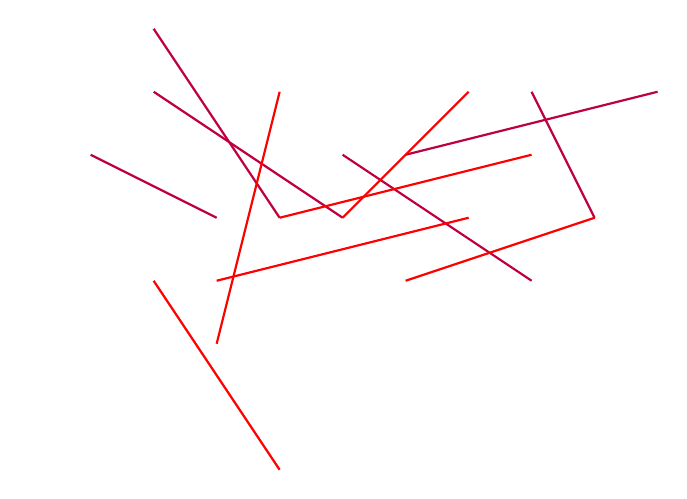
\begin{tikzpicture}[scale=0.8]

% Whiteboard
\fill[white] (0,0) rectangle (10,5);

% Purple Arrows
\draw[thick, purple] (2,4) -- ++(3,-2);
\draw[thick, purple] (4,2) -- ++(-2,3);
\draw[thick, purple] (6,3) -- ++(4,1);
\draw[thick, purple] (8,1) -- ++(-3,2);

% Red Arrows
\draw[thick, red] (2,1) -- ++(2,-3);
\draw[thick, red] (4,4) -- ++(-1,-4);
\draw[thick, red] (6,1) -- ++(3,1);
\draw[thick, red] (8,3) -- ++(-4,-1);

% Additional Arrows for Dynamism
\draw[thick, purple] (1,3) -- ++(2,-1);
\draw[thick, red] (7,4) -- ++(-2,-2);
\draw[thick, purple] (9,2) -- ++(-1,2);
\draw[thick, red] (3,1) -- ++(4,1);

\end{tikzpicture}
\end{document}